% https://github.com/itu-devops/lecture_notes/blob/master/REPORT.md
\pagenumbering{arabic}
\section{System's Perspective}
\label{system-perspective}

\subsection{Design of MiniTwit-Go}
We use GitHub Actions to manage our CI/CD setup. When a developer makes a change to the code and makes a pull request, a new GitHub Action is invoked. To host our compute virtual machines and store data we used Digital Ocean as our Cloud Provider. A Docker image defines the containerization of the MiniTwit application, the API, logging and monitoring and database, marked as the cluster in Figure \ref{fig:design}.


\begin{figure}[ht]
		\centering
		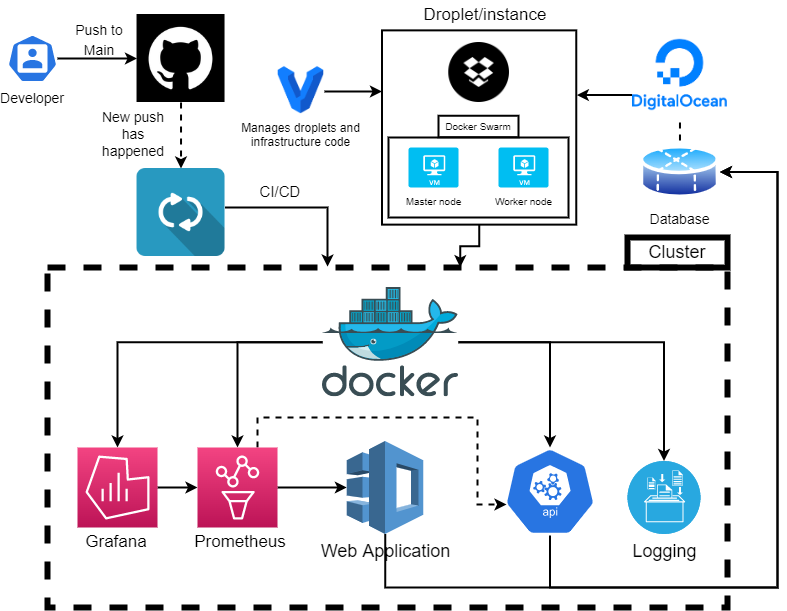
\includegraphics[width=\textwidth]{images/devops_3_design.png}
		\caption{Complete design of the MiniTwit-Go system}
		\label{fig:design}
\end{figure}
	
\subsection{Architecture of MiniTwit-Go}
Figure \ref{fig:packagediagram} shows a top-level diagram of the overall packages in the system. Furthermore, the dependencies between the packages are shown in the diagram. The list below describes and motivates the purpose of each package in the package diagram:

\begin{itemize}
    \item \textbf{Models}: The model is the most dependable package in the system since it is the interface that defines the data to be displayed in the user interface. The data defined here are \textit{structs} that in Go are typed collections of fields, which is useful for grouping data together to form records such as LoginForm for forms and Message for users.
    \item \textbf{Web}: The web solely depends on Models and its  responsibility is to visualize data defined in Models. Web defines a stylesheet (CSS file) as well as the login, register and timeline pages.
    \item \textbf{Controller}: The controller depends on both Models and Database as its responsibility is to determine which Web view to display in response to any incoming action, including when the system loads.
    \item \textbf{API}: The API solely depends on Models since its responsibility is to use and call the application defined data in Models, and does not depend on any other package. 
    \item \textbf{Database}: The database depends on the controller and is responsible for long term storage.
\end{itemize}

\begin{figure}[ht!]
		\centering
		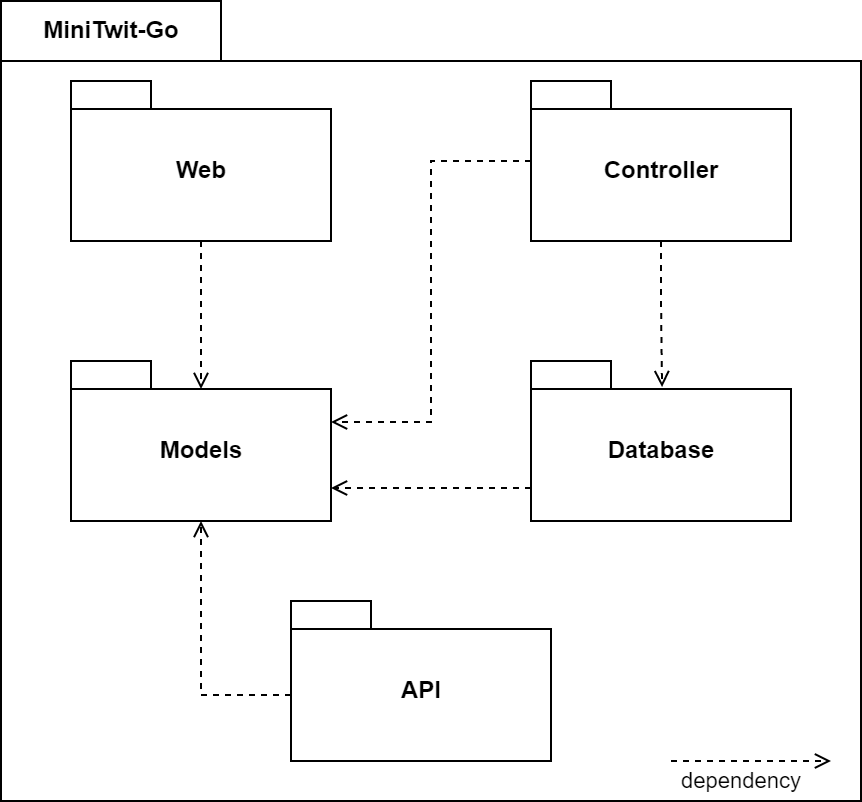
\includegraphics[width=0.7\textwidth]{images/packagediagram.png}
		\caption{Package diagram of the MiniTwit-Go System}
		\label{fig:packagediagram}
\end{figure}

%All dependencies of your ITU-MiniTwit systems on all levels of abstraction and development stages.
    %That is, list and briefly describe all technologies and tools you applied and depend on.
\subsection{Dependencies of our system}
Below is a list and a brief description of all the technologies and tools we applied and are dependent on:

\begin{itemize}
    \item \textbf{Go}: We chose Google's relatively new programming language Golang since it is good for developing web applications, easy to maintain, and faster than many other programming languages. It is often compared to C in terms of speed and efficiency. Furthermore, Go does not require an interpreter, freeing up power and boosting performance. Lastly, there was a wish of working with Golang as it is a new programming language that no one within the group has worked with before \cite{whyusego}.
    \item \textbf{Gin Framework}: We chose Gin because it is a high-performance Golang framework for creating web applications and contains a lot of useful modules. Furthermore, it reduces boilerplate code by providing commonly used functionalities, such as routing, middleware support, rendering, etc. Thus, it makes it easier to build web applications \cite{gin}. 
    \item \textbf{DigitalOcean}: We chose DigitalOcean because it is coupled with the GitHub education pack. DigitalOcean provides free credits, which is advantageous for us as students. Furthermore, it is a simple cloud service provider that is suitable for small applications and projects and simple to setup. The documentation for DigitalOcean is straightforward and comprehensible to get started quickly. 
    \item \textbf{Vagrant}: Vagrant was chosen since combining DigitalOcean with Vagrant provides a clean way to boot up virtual machines to host our web application. In short, Vagrant can be seen as a scripting engine for VirtualBox. Another point is that it can be source controlled with ease since everything is defined in a single text file. You can of course version control a snapshot of the virtual machine, but that will take up a lot more space than just a Vagrantfile.
    \item \textbf{GitHub Actions}: We first went with Travis CI but changed to GitHub Actions, simply because Travis was going to start charging for its usage. 
    \item \textbf{GORM (ORM library)}: This library was chosen because its the main ORM (Object-Relational Mapping) library for Golang. Moreover, it allowed us to automatically migrate schemas which would automatically create tables based on our model. Finally, GORM is developer-friendly and well documented, which makes it easy to work with. 
    \item \textbf{Docker Swarm}: A separate tool within Docker that manages and orchestrates "swarms" of Docker containers. It is useful for providing scaling and load balancing strategies.
    \item \textbf{ELK stack (Kibana, filebeat, elasticsearch)}: A stack of data analytic tools for collecting, processing, and visualizing system log output.
    \item \textbf{Prometheus and Grafana}: Prometheus is a monitoring system and alerting toolkit used for monitoring our virtual machines. Grafana is an analytic and interactive visualization web application that provides queries, clear presentation through charts and graphs, and customizable dashboards. The output of Prometheus can be used as input to Grafana to produce analytic data.
    \item \textbf{Bugsnag}: An error-monitoring tool used to identify, prioritize and replicate bugs found in our system. Helps us as developers to easier spot the effects of our code and address issues before they escalate.
    \item \textbf{DuckDNS}: A dynamic DNS service that points a DNS to an IP of our choice. It eliminates the need to remember a specific IP address.
\end{itemize}

\subsection{Important interactions of subsystems}   

An example where we have an interaction between some of the subsystems in MiniTwit-Go is when the user registers through the frontend. The logic is sent to the \textit{registration.go} module in the Controller package, which uses the model from the Models package and updates the information in the database. This way we can separate our logic into different functionalities and put them in a separate subsystem. This can be seen in Figure \ref{fig:subsysteminteraction}. 

\begin{figure}[ht]
		\centering
		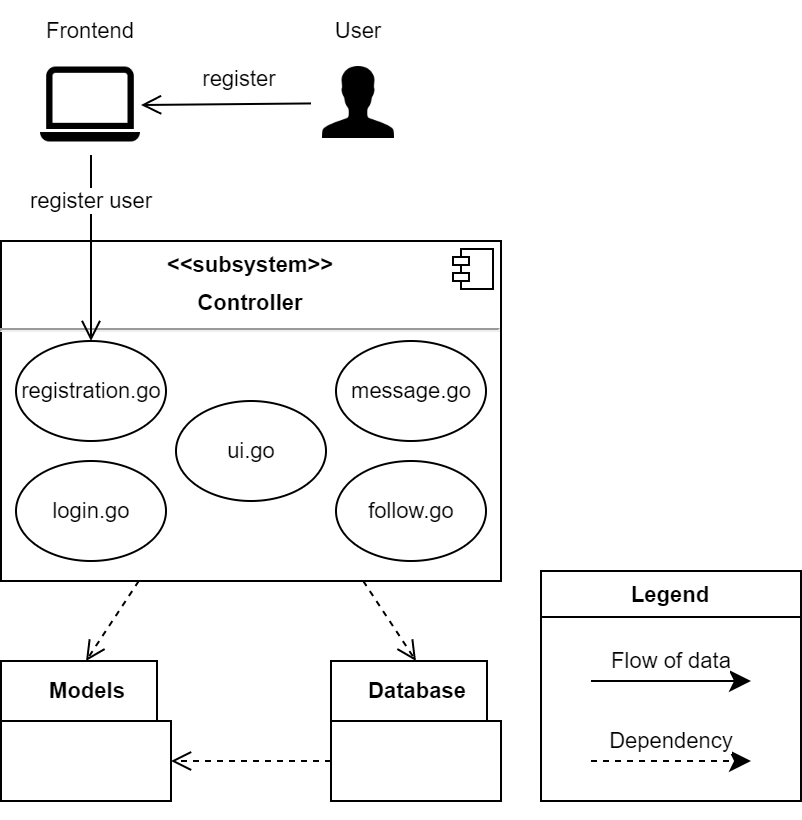
\includegraphics[width=0.5\textwidth]{images/subsysteminteraction.png}
		\caption{User registration shown with interaction of subsystem}
		\label{fig:subsysteminteraction}
\end{figure}

%Describe the current state of your systems, for example using results of static analysis and quality assessment systems.
\subsection{Current state of Minitwit-Go}
The system will be assessed with the 3 focus points: \textbf{operability}, \textbf{simplicity}, \textbf{evolveability} from Kleppmann' definition of software maintainability \cite{Kleppmann17}. The state of the program will be described from a developer perspective, which is the focus of Kleppmann's maintainability operationalization of the term. 

\begin{itemize}
    \item \textbf{Operability} - \textit{Making Life Easy for Operations}:
    \begin{itemize}
        \item \textbf{Health monitoring}: we use Prometheus for storing times series data about the health of our system and Grafana for visualising them
        \item \textbf{Cause of issues}: Bugsnag helps us detect code bugs and their origin and automatically creates GitHub Issues. Whereas the Grafana gives an overview of the performance e.g., CPU usage, memory usage etc. Finally Elasticsearch stores logs from our service and through Kibana it is possible to visualize them and filter and research them.
        \item \textbf{Automation and integration of tools}: We use GitHub Action to ensure automatic Continuous Integration (with several static analysis tool) and Continuous Deployment. Every time a pull request is merged into the \textit{main} branch, the new version of the system is deployed into production and a new release is published on GitHub.
        \item \textbf{Single point of failure}: We have a single point of failure on the manager node of Docker Swarm. If the Docker service in the manager virtual machine stops working that would make the entire infrastructure stop working. To ensure High Availability and avoid Single-point of failure we should have multiple manager nodes, which we have avoided because of the cost. 
        \item \textbf{Documentation}: The entire system is well-documented everything from deployment to configuration of the individual components. 
        \item \textbf{Self-healing/roll-back mechanism}: We don't have any automatic roll-back mechanism, however, since any image is tagged with the GitHub workflow build number, it is easy to roll back to the previous working version. Docker Swarm ensures self-healing techniques such as restarting a container in case of failure.
    \end{itemize}
    \item \textbf{Simplicity} - \textit{Managing Complexity}
    \begin{itemize}
        \item \textbf{Tight coupling vs loose coupling}: All of our components are built independently, even though they might rely on others to work (e.g. API and Web-App rely on Database, Kibana rely on Elasticsearch etc.)
    \end{itemize}
    \item \textbf{Evolvability} - \textit{Making Change Easy} 
    \begin{itemize}
        \item How easy is the system to change: as most of the components are loosely coupled in the architecture it is relatively easy to substitute the individual components.  
    \end{itemize}
    
\end{itemize}

\paragraph{Quality assessment}
From Arachni we did a quality assessment of our API\footnote{An interactive dashboard can be found here: \url{https://www.arachni-scanner.com/reports/report.html/\#!/summary/charts}}. Apart from the penetration part, which we will touch upon later, more \textit{interesting} was the HTTP not-expected responses e.g., sometimes we get a 200-OK when we should not. These issues explain some of the issues we had with the API simulation test during the course \footnote{The entire report can be found at \url{https://github.com/ITU-DevOps-N/go-minitwit/pen_report.html}}. 
In short, we still have some issues with our code, which we at this point have not managed/prioritized to fix.



\subsection{License}
To scan our project for licenses of our dependencies we used Lichen\footnote{https://github.com/uw-labs/lichen}. The dependencies of our project use the licenses: MPL-2.0, Apache-2.0, BSD-3-Clause and BSD-2-Clause. All these aforementioned licenses are compatible with the MIT-license of our project, which means we can bundle all the licenses together under the MIT license. 